% ============================================================================
%  Minor Project Report — RFI detection in radio spectrograms
%  Ronak Singh, IMS23319, School of Physics, IISER Thiruvananthapuram
%
%  Build:   latexmk -pdf main.tex        (clean: latexmk -C)
%
%  HOW THIS SKELETON WORKS
%  Every chapter file in chapters/ holds the headings plus an outline written
%  as LaTeX comments (lines starting with %). Comments never appear in the
%  PDF. Write your own paragraphs underneath each outline block, then delete
%  the outline once the section is done.
%
%  Every number in an outline is followed by [source: ...]. Those sources
%  are files in this repo or PARTs of RFI-project-context.md. If you add a
%  number that has no source, it should not go in the report.
% ============================================================================
\documentclass[12pt,a4paper,oneside]{report}

% ---- page and fonts --------------------------------------------------------
\usepackage[margin=2.5cm]{geometry}
\usepackage[T1]{fontenc}
\usepackage[utf8]{inputenc}
\usepackage{lmodern}
\usepackage{microtype}
\usepackage{setspace}
\onehalfspacing

% ---- maths, tables, figures ------------------------------------------------
\usepackage{amsmath,amssymb}
\usepackage{siunitx}
\usepackage{booktabs}
\usepackage{multirow}
\usepackage{graphicx}
\graphicspath{{figures/}}
\usepackage{caption}
\usepackage{subcaption}
\usepackage{float}

% ---- code listings (for the one or two snippets worth showing) -------------
\usepackage{xcolor}
\usepackage{listings}
\lstset{basicstyle=\ttfamily\small, breaklines=true, frame=single,
        columns=fullflexible, keepspaces=true}

% ---- references ------------------------------------------------------------
\usepackage[numbers,sort&compress]{natbib}
\bibliographystyle{unsrtnat}

% ---- links (load last) -----------------------------------------------------
\usepackage[hidelinks]{hyperref}
\usepackage[nameinlink,capitalise]{cleveref}

% ---- house style -------------------------------------------------------------
% Use these so terms are spelled the same everywhere.
\newcommand{\tfunet}{\texttt{tf\_unet}}
\newcommand{\hybrid}{HybridRFINet}
\newcommand{\aoflagger}{\textsc{AOFlagger}}
\newcommand{\Fone}{$F_1$}

% ============================================================================
\begin{document}

% ---- title page --------------------------------------------------------------
\begin{titlepage}
  \centering
  \vspace*{1cm}
  {\Large Indian Institute of Science Education and Research\\Thiruvananthapuram\par}
  \vspace{2cm}
  {\huge\bfseries Detecting Radio Frequency Interference in\\[0.3em]
   Radio Spectrograms with Convolutional Networks\par}
  % TODO: the title should match what your project is finally about. Decide
  %       after the meeting on novelty -- see chapters/01_introduction.tex.
  \vspace{1.5cm}
  {\Large Minor Project Report\par}
  \vspace{2cm}
  {\large Ronak Singh\\IMS23319\\BS-MS, 4th Year\\School of Physics\par}
  \vspace{1.5cm}
  {\large Supervisor: \textit{TODO}\par}
  \vfill
  {\large TODO month 2026\par}
\end{titlepage}

\pagenumbering{roman}

% ---- certificate / declaration --------------------------------------------
% TODO: IISER-TVM usually requires a supervisor certificate and a student
%       declaration. Ask the department for the exact wording.

\chapter*{Abstract}
\addcontentsline{toc}{chapter}{Abstract}
% Write this LAST. ~200 words. One sentence each:
%  - the problem (RFI corrupts radio data; flagging it is a segmentation task)
%  - what you did (reproduced tf_unet, diagnosed its failure, built a model,
%    tested on synthetic + real LOFAR data with human labels)
%  - the main numbers (tf_unet 0.39 -> 0.93 synthetic; on LOFAR your model
%    0.6603 +/- 0.0040 vs best published 0.5979) [source: PART 1, PART 13.11]
%  - the honest finding (the gain is not from the added components) [PART 20]
%  - why it matters (synthetic benchmarks overstate real performance by 0.38)

\chapter*{Acknowledgements}
\addcontentsline{toc}{chapter}{Acknowledgements}
% Thank your supervisor and the DIL lab.
% Keep this disclosure (or your own wording of it):
Parts of the data analysis, figure generation and drafting support for this
report were carried out with the assistance of Claude (Anthropic). All
experiments, results and conclusions are the author's own.

\tableofcontents
\listoffigures
\listoftables

\clearpage
\pagenumbering{arabic}

\chapter{Introduction}
\label{ch:intro}

\section{Radio frequency interference}
% - Radio telescopes record extremely weak signals from space. Human-made
%   transmitters (mobile networks, satellites, aircraft, broadcast, electrical
%   equipment) are millions of times stronger. This is RFI.
% - RFI corrupts the data. It has to be found and removed ("flagged") before
%   any science is done. Your Week-2 slides cover the RFI types: constant
%   narrowband lines, constant broadband bands, instantaneous wideband bursts,
%   patchy broadband blobs -- reuse that, with the figure.
% - Telescopes produce far too much data to flag by hand, so flagging must be
%   automatic.
% - Original motivation from your Week-2 deck: GMRT pulsar timing for InPTA,
%   where uncleaned RFI damages sub-microsecond timing precision.

\section{RFI flagging as image segmentation}
% - A spectrogram is a 2D image: one axis time, one axis frequency, each
%   pixel a measured power.
% - Flagging = deciding, for every pixel, "RFI or not". That is exactly the
%   task computer-vision people call semantic segmentation.
% - U-Net (Ronneberger et al. 2015) is the standard segmentation network.
%   Akeret et al. 2017 were the first to apply it to RFI: tf_unet.
% - Classical alternatives: thresholding, AOFlagger (Offringa et al. 2012),
%   the 2-sigma CRF method (Chen et al. 2023). Details in Chapter 2.

\section{Aims of this project}
% Say what you set out to do, in the order you actually did it:
%  1. Reproduce the authors' tf_unet on our own data.
%  2. Understand why it performed badly (F1 0.39) and fix it.
%  3. Build an improved model.
%  4. Test both on REAL telescope data with human ground truth (LOFAR),
%     not only on synthetic data.
%  5. Find out what actually makes the improved model better.

\section{Contributions}
% TODO -- DECIDE THIS AFTER THE NOVELTY DISCUSSION WITH YOUR SUPERVISOR.
% This section sets the argument of the whole report. Candidates, all backed
% by measurements:
%  - Diagnosis of tf_unet's failure: class weighting + the ReLU output layer
%    drive it into a dead state; per-image normalisation does the rest.
%    0.3879 -> 0.9317 without changing the model. [PART 1]
%  - A 593,842-parameter model scoring 0.6603 +/- 0.0040 max F1 on the 109
%    expert-labelled LOFAR baselines, above the best published result
%    (RFI-Net, 0.5979). [PART 13.11, PART 14]
%  - Evidence that the gain does NOT come from the added architectural
%    components (strip convolutions, ECA, residual blocks). [PART 18, 20]
%  - Dataset audits: train/test leakage in the published HERA split (31 of
%    140 test images) and in the LOFAR split (all 109 test images). [PART 2, 11.5]
%  - The synthetic-to-real gap: identical code drops 0.9317 -> 0.5482. [PART 12]
% Do NOT claim the strip-convolution idea as novel: prior art MARS,
% arXiv:2608.05546 [PART 4].

\section{Structure of this report}
% One line per chapter. Write last.

\chapter{Background}
\label{ch:background}

\section{RFI in spectrograms}
\label{sec:rfi_types}
In a spectrogram, different kinds of RFI leave different shapes, depending on
how long they last and how many frequencies they cover.
\begin{itemize}
  \item \textbf{Constant narrowband RFI} affects a single frequency channel for
    the whole observation and appears as a thin line along the time axis.
    Typical sources are fixed terrestrial transmitters, such as a particular
    radio or television station.
  \item \textbf{Constant broadband RFI} covers a wide range of frequencies for the
    whole observation and appears as a thick band. Continuously broadcasting
    satellites are a common cause.
  \item \textbf{Instantaneous wideband RFI} lasts only a moment but covers almost
    all frequencies, appearing as a thin line along the frequency axis.
    Lightning, arcing on power lines and radar sweeps produce this kind.
  \item \textbf{Patchy broadband RFI} covers several channels for a few minutes
    and then fades, appearing as irregular, cloud-like patches.
\end{itemize}
Not every structure in a spectrogram is RFI. The receiver's sensitivity
varies with frequency (the bandpass, \cref{sec:bandpass}), and slow drifts and
standing waves add smooth patterns. A flagging method has to distinguish these
from real interference.

\section{Classical flagging methods}

\subsection{Statistical thresholds}
The simplest approach flags any pixel more than $k$ standard deviations above
the mean. Tools used for folded pulsar data, such as \texttt{paz} and
\texttt{clfd}, are based on robust statistics of this kind, such as medians.
They need no training, but they assume the clean data is close to Gaussian, so
they miss faint RFI and struggle when the noise level changes across the data.
On the LOFAR test data, the best simple threshold of this kind reaches an
\Fone{} of 0.41 (\cref{sec:tfunet_lofar}).

\subsection{AOFlagger}
\aoflagger{}~\cite{offringa2012} is the standard RFI flagger for LOFAR. It
combines thresholding at several scales with a morphological step that
extends flags along time and frequency, so that the edges of RFI features are
also caught. It is important for this report because it produced the
training labels of the LOFAR dataset (\cref{sec:lofar}).

\subsection{The 2\texorpdfstring{$\sigma$}{-sigma}CRF method}
Chen et al.~\cite{chen2023} clean RFI in folded pulsar data in two steps.
First, they compute the root-mean-square of the folded profile in each
frequency channel and time sub-integration, giving a 2D image, remove its
baseline, and fit a Gaussian to the histogram of its values. Pixels within
$2\sigma$ of the Gaussian peak are labelled clean, pixels beyond $3\sigma$ are
labelled RFI, and those in between are left ambiguous. Second, they refine
these labels with a fully connected conditional random field
(CRF)~\cite{krahenbuhl2011}. A CRF treats every pixel as connected to the
others and finds the labelling that minimises an energy made of two parts: a
unary term, how likely each pixel is to be RFI on its own, and a pairwise
term, which encourages pixels that are close together and similar in value to
share a label. This lets weak RFI that is unrecognisable in a single pixel be
picked out from its neighbourhood. They report 93--95\% accuracy on data from
the FAST telescope. The method still rests on a Gaussian model of the clean
data, which is where a learned approach might do better.

\section{Neural networks for RFI segmentation}

\subsection{U-Net}
The U-Net~\cite{ronneberger2015} is a convolutional network for image
segmentation. Its encoder repeatedly applies convolutions and halves the image
size, building up a description of \emph{what} is in the image; its decoder
reverses this, restoring the full size to locate \emph{where} it is. Skip
connections pass fine detail directly from each encoder level to the matching
decoder level. The output has one probability per pixel---here, the
probability that the pixel is affected by RFI.

\subsection{\tfunet{}}
Akeret et al.~\cite{akeret2017} applied a U-Net to RFI in their \tfunet{}
code, written in TensorFlow. The configuration used in this report has 3
levels and 32 filters in the first layer, giving 465{,}986 trainable
parameters. Two design details become important later: \tfunet{} applies a ReLU
to its output scores, and it has no normalisation layers
(\cref{ch:tfunet}).

\subsection{Recent methods}
Mesarcik et al.~\cite{mesarcik2022}, who released the LOFAR dataset used here,
proposed an approach called Nearest-Latent-Neighbours, which learns only from
RFI-free data and flags whatever looks unusual. They compared it with several
supervised networks on the same LOFAR test set. The best \Fone{} in their
comparison came from RFI-Net~\cite{yang2020rfinet}, a residual U-Net, with
0.5979; their own U-Net reached $0.5876 \pm 0.0031$. Their method had the best
area under the ROC curve but a lower \Fone{} of 0.5114. These published values
are the benchmarks used in \cref{ch:hybrid}.

\section{Measuring performance}
\label{sec:metrics}
For each pixel, a flagging method either flags it as RFI or not, and it either
is or is not RFI in the reference labels. Counting the true positives (TP),
false positives (FP) and false negatives (FN) over all test pixels gives
\begin{equation}
  \text{precision} = \frac{TP}{TP + FP}, \qquad
  \text{recall} = \frac{TP}{TP + FN}, \qquad
  F_1 = \frac{2\,\text{precision}\cdot\text{recall}}{\text{precision} + \text{recall}}.
\end{equation}
Precision is the fraction of flagged pixels that really are RFI; recall is the
fraction of RFI that was found. \Fone{} is high only if both are.

Accuracy, the fraction of pixels classified correctly, is not useful here.
RFI covers less than 1\% of the LOFAR test pixels, so a method that flags
nothing at all is 99.23\% accurate while finding no RFI.

The area under the ROC curve measures something different: how well a model
\emph{ranks} RFI pixels above clean ones, regardless of where the final cut is
made. A model can rank well and still make poor final decisions
(\cref{sec:hybrid_lofar}).

\paragraph{Choosing the threshold.} A network outputs a probability for each
pixel, and a threshold turns it into a yes/no decision. The choice of threshold
changes the \Fone{}, and there are two ways to make it.
\begin{itemize}
  \item \textbf{Maximum \Fone{}:} try every threshold on the test set and report
    the best. This is optimistic, because it uses the test labels to pick the
    threshold. It is, however, what Mesarcik et al.\ report, so it is needed
    for a fair comparison with their results.
  \item \textbf{Pooled \Fone{}:} choose the threshold on a separate validation
    set, fix it, and then apply it to the test set. This is the honest
    measure of how a model would perform on new data.
\end{itemize}
For example, if a model scores ten pixels and the best threshold on those ten
gives $F_1 = 0.89$, but the threshold chosen beforehand on validation data
gives $0.86$ on the same pixels, the maximum \Fone{} is 0.89 and the pooled
\Fone{} 0.86. The maximum is never lower than the pooled value. In this report
both are given; the pooled value is the one I rely on.

``Pooled'' also means that TP, FP and FN are added up over all test images
before computing a single \Fone{}. Averaging a separate \Fone{} for each image
gives a different number: for \aoflagger{} on LOFAR, the per-image average is
0.103 lower than the pooled value.

\chapter{Datasets}
\label{ch:datasets}
% Opening paragraph: four datasets, two synthetic (ours), two from the
% literature. Only LOFAR has real telescope data with human labels -- say up
% front that this is the one that matters most.

\section{Synthetic dataset}
\label{sec:synthetic}
% Write about your generator. Sources: PART 8, PART 9, "Verified facts"
% section of the context doc, Synthetic Dataset*/dataset_statistics.txt.

\subsection{Generation}
Real radio data with reliable pixel-level RFI labels is scarce, so the first
part of this work used a synthetic dataset that I generated myself. The
generator is written in Python and uses NumPy's random number generator with a
fixed seed (42), so the whole dataset can be regenerated bit for bit.

Each image is a spectrogram: one axis is frequency and the other is time, and
each pixel holds the power received in that frequency channel at that moment.
The background is not plain random noise. It is built from a sky pedestal that
varies across frequency, a smooth astronomical signal, a slow drift in time,
and Gaussian noise on top. RFI is then injected into this background. Six
types of RFI are modelled, chosen to cover the shapes commonly seen in real
observations (\cref{tab:rfi_types}). Each image receives a random selection of
types at random strengths, and images are spread over four density levels:
clean (8.2\%), light (30.0\%), moderate (36.2\%) and heavy (25.6\%).

\begin{table}[H]
  \centering
  \caption{The six RFI types in the synthetic dataset, with the number of the
    1000 images (1024$\times$265 version) that contain each type.}
  \label{tab:rfi_types}
  \begin{tabular}{llr}
    \toprule
    Type & Appearance in the spectrogram & Images \\
    \midrule
    Narrowband      & thin line at one frequency, lasting for some time  & 889 \\
    Scattered       & small isolated hits scattered over the image        & 899 \\
    Blob            & patchy, cloud-like region                           & 673 \\
    Persistent band & group of channels affected for the whole observation & 588 \\
    Broadband block & rectangle covering many channels for a while        & 488 \\
    Wideband burst  & short flash across many channels at once            & 310 \\
    \bottomrule
  \end{tabular}
\end{table}

The dataset contains 1000 images, split into 700 for training, 150 for
validation and 150 for testing. I checked that no image appears in more than
one split by comparing SHA-256 hashes of the raw pixels; there are no shared
hashes.

\subsection{Deciding which pixels are RFI}
\label{sec:synthetic_label}
Because the RFI is injected by the generator, its exact strength at every
pixel is known. A pixel is labelled as RFI when the injected RFI power there
is greater than 0.5 times the standard deviation of the local noise. Pixels
where RFI was added but is weaker than this are labelled clean, because at
that level there is effectively nothing left in the data for a detector to
find.

This rule gives labels that are noise-free and unambiguous: every labelled
pixel is, by construction, measurably above the noise. In the 276$\times$600
version, 90.9\% of the RFI pixels lie at or above one noise standard
deviation. This makes the task considerably easier than labelling real data,
a point that becomes important in \cref{ch:drivers}.

The rule was refined between the two versions of the dataset. In the
276$\times$600 version a pixel was labelled RFI if it lay inside the geometric
outline of an injected RFI shape \emph{or} exceeded the 0.5$\sigma$ threshold.
Because this was a union, it could mark pixels that carried almost no RFI
power (0.06\% of labelled pixels in the training split, and up to 4.49\% in
the worst single image). In the 1024$\times$265 version only the threshold is
used, and it is applied \emph{after} the instrument response
(\cref{sec:bandpass}) and against the total local noise of each channel, so
RFI that the instrument has genuinely buried below the noise is not
labelled.

\subsection{Two versions of the dataset}
\label{sec:synthetic_versions}
Two versions of the dataset were used (\cref{tab:synth_versions}). My first
images were 1024$\times$1024 pixels. At that size only one image fitted in a
training batch on the 6\,GB GPU, which made training unstable. Akeret et
al.~\cite{akeret2017} trained \tfunet{} on images of 276$\times$600 pixels, so
I regenerated the dataset at exactly that size to reproduce their setup as
closely as possible. When the image size changes, the RFI shapes have to be
rescaled as well: a blob 40 channels wide covers 3.9\% of a 1024-channel band
but 14.5\% of a 276-channel band. Seven size-dependent parameters of the
generator were therefore scaled in proportion to the image dimensions.

% TODO (ask Ronak): why 1024x265 for the second version? Reason not
% recorded in the repo. Add one or two sentences here.
The second version, 1024$\times$265, adds a model of the receiver's frequency
response, described in the next section.

\begin{table}[H]
  \centering
  \caption{The two versions of the synthetic dataset. Both use seed 42 and a
    700/150/150 split.}
  \label{tab:synth_versions}
  \begin{tabular}{lccc}
    \toprule
    Version & Size (freq $\times$ time) & Instrument bandpass & RFI pixels \\
    \midrule
    v3 & 276$\times$600  & no  & 14.67\% mean (test split 15.08\%) \\
    v4 & 1024$\times$265 & yes & 14.19\% mean \\
    \bottomrule
  \end{tabular}
\end{table}

\subsection{The instrument bandpass (v4)}
\label{sec:bandpass}
% - Real receivers do not amplify all frequencies equally. Formula
%     B(f) = max( W(f) * [1 + R(f) + S(f)], B_floor )
%   W = Tukey edge taper, R = slow ripple, S = standing wave.
%   [PART 9; code dataset_v4_bandpass/generate_dataset_v4.py]
% - spectrogram = B(f) * (sky + RFI) + receiver noise. Noise is added AFTER
%   the gain, as in a real receiver chain.
% - HONESTY: each ingredient is standard and citable, but the combined
%   formula is ours. Say so. Cite Harris 1978 (Tukey window), Popping & Braun
%   2008 (standing waves), Hamaker et al. 1996 (measurement equation).
%   [PART 9 PROVENANCE]

\section{HERA dataset}
\label{sec:hera}
% - Simulated HERA data from Mesarcik et al., Zenodo 6724065.
%   420 train + 140 test, 512x512, boolean masks, 2.75% RFI. [PART 2]
% - FINDING: the published split leaks. Verified by SHA-256 over raw pixels:
%   382/420 unique train, 135/140 unique test, 31 test images identical to
%   training images = 22% of the test set. [PART 2]
% - After deduplication: 351 train / 135 test / 0 overlap. [PART 3]
% - Mention briefly that it turned out too easy to be informative (models
%   at 0.999 F1) [PART 3] -- but only if you discuss HERA results at all.

\section{LOFAR dataset}
\label{sec:lofar}
% Sources: PART 10, PART 11. Figures: analysis/lofar_analysis/fig_lofar_overview.png
% and fig_lofar_profiles.png already exist.

\subsection{Origin and structure}
% - Real LOFAR observations, Mesarcik et al. 2022, Zenodo 6724065. 9.3 GB.
% - Stored as a Python list of 4 arrays:
%     train images (7500,512,512,1) float32 | train masks (AOFlagger) bool
%     test images  (109,512,512,1)  float32 | test masks (human expert) bool
% - 512x512 is a random crop from 599x616.
% - Rows = time, columns = frequency. You measured this three ways
%   [PART 11.2]: 65-74% of RFI pixels sit in 16 of 512 columns.
%   (Opposite orientation to our synthetic data.)
% - Values are RAW powers, 0 to 1.4e11 -- max is ~39,000x the 99th
%   percentile. That is why plt.matshow shows a flat square. [PART 11.1]

\subsection{Audit}
% Table of what you found [PART 11.3-11.6]:
%  - Imbalance: train 1.27% RFI (1:78), test 0.766% (1:129).
%  - 35 training images are 100% flagged (dead baselines).
%  - All 109 test images are byte-identical to 109 training images.
%    Verified by MD5 and element-wise equality, largest pixel difference 0.
%    Only the labels differ. [PART 11.5; analysis/lofar_analysis/prove_test_set_leakage.py]
%  - Clean training set: 7500 - 109 - 35 = 7356; minus 735 for validation
%    = 6621 used for training.
%  - Training labels vs human labels on the same pixels: F1 0.5698403,
%    matching the paper's published 0.5698 to four decimals. This confirms
%    the data, labels and metric are the same as theirs. [PART 11.6]

\subsection{Why it is harder than the synthetic data}
% - Training labels are ~44% wrong against the human expert.
% - RFI brightness tiers, using each image's own clean pixels as the ruler
%   [PART 15; analysis/ablation_faint_recall.py lines 82-100]:
%     bright 50.1% | moderate 18.9% | faint 11.0% | invisible 20.0%
%   "Invisible" = dimmer than the median clean pixel. No brightness
%   evidence at all -- only context can find it.
% - Explain the bucketing method briefly (you understood it from the
%   step-by-step explanation).
% - Practical note: the pickle does not fit in RAM alongside other work;
%   converted once to memory-mapped arrays (28.7 MB resident). Mention in a
%   sentence, details in the appendix.

\chapter{Reproducing and diagnosing \tfunet}
\label{ch:tfunet}

\section{Initial result}
The first step was to reproduce the authors' method. I used their \tfunet{}
code without modifying the network itself, with 3 layers and 32 features in
the first layer (465{,}986 trainable parameters), and trained it on the
276$\times$600 synthetic dataset. Two settings had to differ from the paper.
Akeret et al.\ used a batch of 32 images and momentum gradient descent with a
learning rate of 0.2~\cite{akeret2017}. A batch of 32 does not fit on the
6\,GB GPU used here, so I used a batch of 4. At such a small batch the paper's
learning rate destroyed the network within a few iterations (with a batch of
one it stopped learning at iteration 4), so I used the Adam optimiser with a
learning rate of $10^{-3}$ instead.

The result was poor: a maximum \Fone{} of only 0.3879 on the test set, while my
own model (\cref{ch:hybrid}) scored about 0.98 on the same data. The obvious
conclusion would have been that the authors' architecture is simply weaker.
My first suspicion was the normalisation of the input images. Rather than
assume either explanation, I ran a set of controlled experiments.

\section{Four controlled runs}
In four runs everything was kept the same---dataset, network, optimiser and
batch size---except two settings: how the input images were normalised, and
whether class weighting was used (\cref{tab:tfunet_runs},
\cref{fig:tfunet_runs}). Class weighting gives the rare RFI pixels a larger
weight in the loss, and had been added by us to deal with the imbalance
between RFI and clean pixels; it is not part of the authors' setup.

\begin{table}[H]
  \centering
  \caption{\tfunet{} on the 276$\times$600 synthetic dataset. Only the
    normalisation and the class weighting change between runs.}
  \label{tab:tfunet_runs}
  \small
  \begin{tabular}{clcrrrl}
    \toprule
    Run & Normalisation & Class weights & Epochs & ROC AUC & max \Fone{} & Behaviour \\
    \midrule
    1 & per-image   & on  & 22 & 0.6681 & 0.3879 & frozen for 15 epochs \\
    2 & per-image   & on  & 5  & 0.5677 & 0.3064 & collapsed, stopped \\
    3 & per-image   & off & 60 & 0.8747 & 0.7191 & trained normally \\
    4 & fixed range & off & 60 & 0.9908 & 0.9317 & trained well \\
    \bottomrule
  \end{tabular}
\end{table}

\begin{figure}[H]
  \centering
  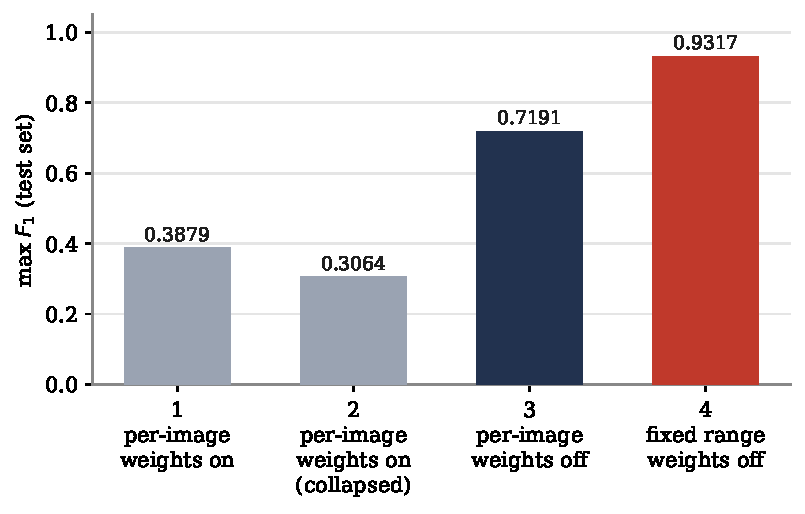
\includegraphics[width=0.75\textwidth]{tfunet_controlled_runs}
  \caption{Test \Fone{} of the four controlled \tfunet{} runs of
    \cref{tab:tfunet_runs}. The network is identical in all four.}
  \label{fig:tfunet_runs}
\end{figure}

Removing the class weights and switching to a fixed normalisation range raised
the score from 0.3879 to 0.9317 without any change to the network. Runs 3 and
4 differ only in normalisation and were trained for the same number of epochs,
so the gain from normalisation alone, $+0.213$, is a fair comparison. The
effect of class weighting is less cleanly separated: run~2 was stopped at
epoch~5 by an automatic check that detects a collapsed network, and run~1
after 22 epochs, while runs 3 and 4 trained for 60. As
\cref{sec:tfunet_v4} shows, a frozen network can eventually recover if
trained for longer, so part of the difference between runs 1--2 and run~3 is
due to training length. What the runs establish clearly is that the poor
initial score came from these two settings, not from the architecture.

\section{Cause 1: class weighting and the ReLU output}
\label{sec:relu_trap}
For every pixel, \tfunet{} produces two scores, one for ``clean'' and one for
``RFI'', and passes both through a ReLU before turning them into
probabilities. A ReLU replaces any negative value with zero. Class weighting
pushes the network strongly towards predicting RFI, which drives the
``clean'' score negative. The ReLU then sets it to exactly zero, and because
the slope of a ReLU is zero for negative inputs, no gradient flows back: the
network has no signal telling it how to change that score. It stops learning.

This is exactly what run~2 shows. It gave the same output, 0.537, for every
one of the 24{,}840{,}000 test pixels. Working backwards through the softmax,
$\mathrm{softmax}(0, c)_2 = 0.537$ gives $c = 0.148$: the ``clean'' score was
stuck at zero and the ``RFI'' score at 0.148 everywhere. The network had become
a constant.

Neither part is a problem on its own. The authors trained successfully with
the ReLU, and class weighting is a standard remedy for imbalanced data. It is
the combination that causes the network to freeze. The freeze is long rather
than permanent: on the second synthetic dataset the same network stayed frozen
for 15 epochs and then began to recover (\cref{sec:tfunet_v4}).

\section{Cause 2: per-image normalisation}
\label{sec:pernorm}
The data loader we had written scaled each image by its own minimum and
maximum. In this dataset the maximum value of an image ranges from 27 to 222,
a factor of 8.2. The same physical brightness therefore ends up at different
values in different images. \Cref{tab:pernorm} shows what this does to a noise
pixel (raw value 10) and a faint RFI pixel (raw value 20).

\begin{table}[H]
  \centering
  \caption{Normalised values of the same two pixels under per-image and
    fixed-range normalisation.}
  \label{tab:pernorm}
  \begin{tabular}{lccc}
    \toprule
    Pixel (raw value) & Per-image, quiet image & Per-image, bright image & Fixed range \\
     & (max 27) & (max 222) & \\
    \midrule
    Noise (10)     & 0.370 & 0.045 & 0.345 \\
    Faint RFI (20) & 0.741 & 0.090 & 0.520 \\
    \bottomrule
  \end{tabular}
\end{table}

With per-image scaling, noise in the quiet image (0.370) appears brighter than
real RFI in the bright image (0.090), so no single threshold separates RFI from
noise across all images. A fixed range keeps the ordering. The authors had
avoided this problem: their own launch script clips every image to the same
fixed range (from 30 to 210), but this was lost when their code was adapted to
our data. \tfunet{} has no normalisation layers inside the network, so it
cannot correct for it.

The fix was to scale all images with one fixed range, taken as the 0.5th and
99.5th percentiles of the pixel values, averaged over 40 training images
(giving $-9.69$ and $47.40$). Percentiles are used rather than the minimum and
maximum because a single extreme pixel can move the minimum or maximum a long
way. Only training images are used, so no information from the test set
enters the normalisation.

\section{The bandpass dataset}
\label{sec:tfunet_v4}
I repeated the two extreme settings on the 1024$\times$265 dataset with the
instrument bandpass. With per-image normalisation and class weights, the
network stayed frozen at a validation \Fone{} of about 0.37 for the first 15
epochs, then escaped and kept improving until the last epoch, finishing at a
test \Fone{} of 0.6815. With a fixed range and no class weights it reached
0.9483 and had converged by epoch 30. The same two settings decide the result
on the harder dataset too.

\section{\tfunet{} on real LOFAR data}
\label{sec:tfunet_lofar}
Having found the settings that make \tfunet{} work on synthetic data, I trained
it on the real LOFAR data with exactly those settings: the unmodified network,
fixed-range normalisation and no class weighting. The model was trained on the
6621 clean training images, the threshold was chosen on the 735 validation
images, and the result was measured on the 109 images labelled by the human
expert. Each setting was run with three random seeds.

Despite the extreme imbalance---one RFI pixel for every 129 clean ones---the
network did not collapse into predicting ``no RFI'' everywhere. With the same
training length as on the synthetic data (60 epochs at a learning rate of
$10^{-3}$) it reached a maximum \Fone{} of $0.4901 \pm 0.0495$. Lowering the
learning rate to $10^{-4}$ and training for 150 epochs raised this to
$0.5482 \pm 0.0139$ (\cref{tab:tfunet_lofar}).

\begin{table}[H]
  \centering
  \caption{\tfunet{} on the 109 human-labelled LOFAR test images. Mean and
    standard deviation over three seeds.}
  \label{tab:tfunet_lofar}
  \begin{tabular}{lccc}
    \toprule
    Training & max \Fone{} & pooled \Fone{} & ROC AUC \\
    \midrule
    lr $10^{-3}$, 60 epochs  & $0.4901 \pm 0.0495$ & $0.4563 \pm 0.0279$ & $0.9389 \pm 0.0045$ \\
    lr $10^{-4}$, 150 epochs & $0.5482 \pm 0.0139$ & $0.5021 \pm 0.0259$ & $0.9470 \pm 0.0074$ \\
    \bottomrule
  \end{tabular}
\end{table}

The lower learning rate also made the result much more consistent between
seeds: the standard deviation of the maximum \Fone{} fell from 0.0495 to
0.0139. However, the improvement itself is not statistically significant with
three seeds. Comparing the runs seed by seed, one of the three seeds actually
became slightly worse, and a paired $t$-test gives $t = 1.54$ with 2 degrees of
freedom, well below the 4.30 needed for significance at the 5\% level. My
first single run had suggested a gain of 0.118; the two further seeds roughly
halved it. I therefore use the lower learning rate as the better default, but
do not claim it as a proven improvement.

Using per-image normalisation instead, the maximum \Fone{} fell to 0.3039, below
even a simple threshold, which confirms on real data the conclusion of
\cref{sec:pernorm}.

\Cref{fig:tfunet_lofar} places the result among published methods. The values
for Mesarcik et al.'s U-Net and for RFI-Net are taken from their
paper~\cite{mesarcik2022}; I did not re-run those methods. Their results are
reported as maximum \Fone{}, which is why that measure is used here.
\tfunet{} clearly beats a simple $\sigma$-clipping threshold (0.4103) but stays
below \aoflagger{} (0.5698), and is 0.039 below Mesarcik et al.'s U-Net (0.5876).
Two known differences in how that U-Net was trained could account for at least
part of the gap: it was trained on small 32$\times$32 patches rather than full
images, and with a different normalisation. I have not tested which of these
matters.

\begin{figure}[H]
  \centering
  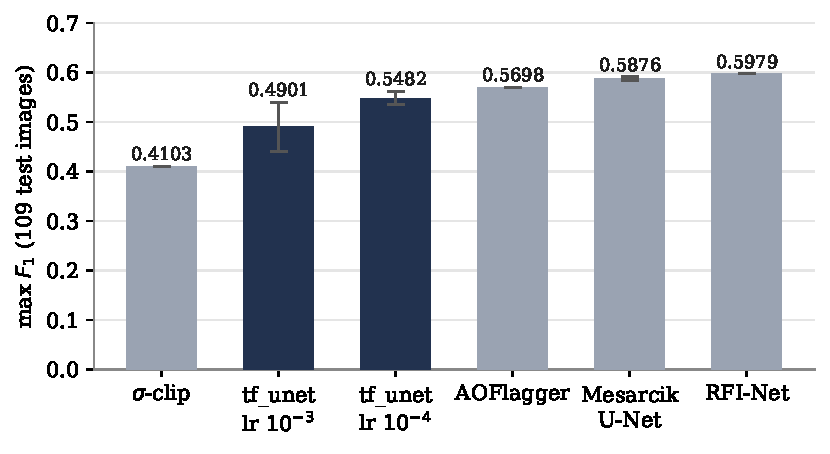
\includegraphics[width=0.8\textwidth]{tfunet_lofar_ladder}
  \caption{Maximum \Fone{} on the 109 LOFAR test images. Dark bars are my
    \tfunet{} runs (error bars: standard deviation over three seeds); grey bars
    are a $\sigma$-clipping threshold, \aoflagger{}, and the values reported by
    Mesarcik et al.~\cite{mesarcik2022}.}
  \label{fig:tfunet_lofar}
\end{figure}

\section{From synthetic to real data}
\label{sec:gap}
The same network, trained with the same settings and the same number of
gradient steps (10{,}500), scores 0.9317 on the synthetic data and 0.4901 on
LOFAR: a drop of 0.44 in \Fone{}. Even the best LOFAR result, after tuning the
learning rate, is 0.38 below the synthetic score. The reasons were set out in
\cref{sec:lofar_harder}: real RFI is far rarer, much of it is fainter than the
noise, and the training labels themselves are often wrong. A method that
performs well on a synthetic benchmark can therefore perform much worse on
real observations, and synthetic results alone should be read with care.

\chapter{\hybrid}
\label{ch:hybrid}
% Framing depends on the novelty decision (see Chapter 1 TODO). Whatever is
% decided, describe the model honestly: these components were ADDED and
% motivated by RFI morphology; Chapter 6 then tests whether they helped.

\section{Architecture}
% Code: src/hybrid_rfi_package/hybrid_model.py. Diagram needed (I can draw it).
% Same U shape as tf_unet. Differences, simply (you have the plain-language
% list from our chat):
%  - Residual blocks: each block learns a change on top of a shortcut.
%  - Multi-scale strip convolutions: 1xK and Kx1 kernels, K = 7, 11, 21,
%    look along long lines in time and frequency. Motivation: RFI is
%    often long thin streaks.
%  - ECA channel attention: re-weights feature channels.
%  - GroupNorm after convolutions.
%  - Raw logits output -- no ReLU on the output layer (avoids Ch. 4 trap).
%  - Same padding -- full 512x512 output.
% Size: base 8 -> 593,842 params; base 32 -> 9,304,186 [PART 6].
% tf_unet for comparison: 465,986.

\section{Training}
% - PyTorch. Loss = cross-entropy + Dice. Adam lr 1e-3, batch 1.
% - 700 steps x 40 epochs = 28,000 gradient steps (same budget as synthetic).
% - Best checkpoint and threshold chosen on 735 validation images.
% - Fixed-range normalisation from training images only.
% [source: experiments/lofar_hybrid.py, run metrics.json]

\section{Results on synthetic data}
% Keep short; synthetic is the easy case.
%  - 276x600: 0.9808 (base 32) [Where the trained models live table]
%  - 1024x265 v4: 0.9878 (base 8)
%  - Width sweep [PART 6]: base 4 0.9547 | base 8 0.9749 | base 16 0.9788 |
%    base 32 0.9812. 15.7x fewer parameters cost only 0.0063.
%    Base 4 genuinely breaks. (These are N=1 -- say so.)

\section{Results on LOFAR}
\subsection{Class weighting}
% - First run used class weights (56.9x on RFI): 0.6467 +/- 0.0079, but a
%   validation threshold of 0.9619 -- badly calibrated. [PART 13.6]
% - Without class weights: 0.6603 +/- 0.0040, threshold 0.2573.
%   Better in every seed, paired t = 6.03 on 2 dof. [PART 13.11]
% - Interesting: ROC fell (0.9801 -> 0.9378) while F1 rose. Ranking and
%   decision quality are different things. [PART 13.13]

\subsection{Final comparison}
% Table, max F1 (the paper's protocol) [PART 13.12]:
%  sigma-clip                  0.4103
%  tf_unet lr 1e-4 (ours)      0.5482 +/- 0.0139
%  AOFlagger                   0.5698
%  Mesarcik et al. U-Net       0.5876 +/- 0.0031
%  RFI-Net (published best)    0.5979
%  HybridRFINet base 8         0.6603 +/- 0.0040   (593,842 params)
% Also give pooled F1: 0.6561 +/- 0.0044 [PART 20 table].
% - +0.0624 over RFI-Net, t = 27.22 on 2 dof.
% - Beats its own teacher: trained on AOFlagger labels (0.5698), scores
%   0.66 against the human.
% - Base 32 at 9.3M params: 0.6571 (N=1, with class weights) -- no gain
%   from 15.7x more parameters [PART 13.7].

\section{Checking the result}
% PART 14 -- an adversarial self-audit. This makes the result credible.
%  - Metrics recomputed by independent code: differences <= 3.2e-5.
%  - Leakage: 0 train/val images in the test set. Normalisation range
%    computed from training images only.
%  - Honest thresholding costs 0.0064 vs choosing on test.
%  - Train/val/test max F1 0.7112 / 0.6820 / 0.6592 -- mild overfitting.
%  - Not copying AOFlagger: agreement with it only 0.7430; finds 16,485
%    true-RFI pixels AOFlagger missed, misses 7,345 it found.
%  - Not a trivial "flag the bad columns" rule: that scores 0.0645.
%  - Bootstrap over the 109 test images (POOLED F1, 2000 resamples):
%    3-seed mean 0.6561, 95% CI [0.6154, 0.6923]. RFI-Net's 0.5979 lies
%    outside; 99.5% of resamples beat it. Note the CI is +/-0.04 wide --
%    the 109-image test set is the biggest source of uncertainty.

\chapter{What drives the performance}
\label{ch:drivers}
% This chapter is what makes the report more than "my model got a higher
% number". You tested your own design and reported what you found.

\section{Ablation on LOFAR}
% Method [PART 17, 18]: experiments/models_ablation.py makes each component
% a switch; experiments/lofar_hybrid.py --variant trains every variant
% through the identical pipeline. Control: the switchable model with
% everything on scored 0.6624 vs the real model's 0.6603 +/- 0.0040.
% Seed 0 table [PART 18.2]:
%   hybrid_full 0.6624 | no_strip 0.6637 | no_eca 0.6557 | no_res 0.6569 |
%   plain_unet 0.6605 | no_groupnorm 0.6289
% 3-seed table [PART 20]:
%   full hybrid    0.6603 +/- 0.0040
%   plain_unet     0.6585 +/- 0.0047   (strip, ECA, residual all removed)
%   no_groupnorm   0.6495 +/- 0.0178   (also no normalisation)
%   Welch t: full vs plain p = 0.64; plain vs no_groupnorm p = 0.48.
% Conclusion: the three added components contribute nothing measurable.
% GroupNorm's effect is not established either -- seed 0 suggested a large
% effect that vanished at 3 seeds. Without GroupNorm, training is less
% stable (sd 0.0178 vs ~0.004).

\section{Do strip convolutions help faint RFI?}
% - The design claim: strips integrate along lines so faint RFI becomes
%   detectable. Overall F1 can't test this (faint RFI is a small share),
%   so you measured recall per brightness tier.
% - First attempt was misleading: each model at its own threshold showed
%   ~+0.02 for strips in the dim tiers -- but hybrid_full's threshold was
%   0.296 vs no_strip's 0.434, and a lower threshold raises recall
%   everywhere. [PART 18.5]
% - Re-done at matched budget (every model flags exactly 199,951 pixels):
%   bright -0.0053 | moderate +0.0029 | faint -0.0008 | invisible +0.0008.
%   No effect anywhere. [analysis/ablation_faint_recall.py]
% - Worth a sentence on the lesson: compare models at the same operating
%   point.

\section{Testing a CRF refinement}
% [PART 16] Chen et al.'s CRF idea, built as a differentiable layer on top
% of the trained network (11 extra parameters).
%  - Chen et al.'s own parameters: 0.6592 -> 0.4884 (destroys thin RFI).
%  - Best hand-tuned: +0.0012. Trained end-to-end: +0.0012 (0.29 seed sd).
%  - Given freedom, the CRF shrank its own weights toward zero.
%  - Why: the network already uses neighbourhood context, and a CRF can only
%    redistribute evidence that is already in the prediction.

\section{Where the remaining errors are}
% [PART 15] Recall by tier for the best model:
%   bright 0.937 | moderate 0.391 | faint 0.268 | invisible 0.254
% - Bright RFI is solved; the dim half is caught only a quarter to a third
%   of the time.
% - Largest possible gain: removing false positives (+0.114 upper bound);
%   perfectly catching the invisible tier (+0.098).
% - And recall the ceiling: training labels are ~44% wrong.

\section{So what does explain the gain over \tfunet?}
% [PART 20.2] Not the three components and not clearly GroupNorm. Still
% untested and confounded: Dice loss, raw-logit output (no ReLU), same
% padding, depth/width, batch size, learning rate, framework.
% Be direct: this is not yet known, and say which experiment comes next
% (start with the Dice loss).

\chapter{Discussion}
\label{ch:discussion}

\section{Synthetic benchmarks can mislead}
% - Same code scores 0.9317 on our synthetic data and 0.5482 on LOFAR.
% - The synthetic label is noise-free (> 0.5 sigma by construction); real
%   labels are noisy and a fifth of real RFI has no brightness signal.
% - Components that look reasonable on paper did nothing on real data, and
%   the earlier synthetic ablation was too noisy to show it either.

\section{Lessons about measurement}
% Three times in this project a single run overstated an effect that
% shrank or vanished with more seeds:
%   lr 1e-4 gain  +0.118 (1 seed) -> +0.058, not significant (3 seeds) [PART 12.10]
%   GroupNorm     -0.0335 (1 seed) -> -0.009, p = 0.48 (3 seeds)       [PART 20]
%   strips on faint RFI: ~+0.02 at own thresholds -> 0 at matched budget [PART 18.5]
% Also the tf_unet failure itself was first blamed on the architecture.
% This section is about method; keep it short and factual.

\section{Limitations}
% [PART 14.8] -- state all of these plainly:
%  1. Published baselines (RFI-Net, their U-Net) are QUOTED from Mesarcik
%     et al. Table 2, not re-run. Our AOFlagger number matches theirs to
%     four decimals, so the test data and metric are the same -- but write
%     "as reported by Mesarcik et al. (2022)".
%  2. 109 test images: +/-0.04 bootstrap interval. Biggest uncertainty.
%  3. Training budgets differ from theirs (they: 32x32 patches, 100 epochs;
%     us: full images, 28,000 steps).
%  4. 3 seeds is the minimum; several conclusions rest on it.
%  5. tf_unet has not been run on HERA.
%  6. The gain over tf_unet is not yet attributed (Chapter 6).

\section{Future work}
% Depends on the novelty discussion. Measured candidates:
%  - Isolate the Dice loss (one run, ~25 min) [PART 19.2].
%  - Reduce false positives -- the largest measured headroom (+0.114).
%  - Apply to GMRT pulsar data (the original motivation).

\chapter{Conclusion}
\label{ch:conclusion}
% Half a page. Write it last. Answer the aims from Chapter 1 one by one,
% each with its number. No new results here.


\appendix
\chapter{Reproducibility}
\label{app:repro}
% This appendix can be mostly tables -- I can fill it for you.

\section{Computing environment}
% - Moved from Windows 11 + WSL2 to a Fedora 44 dual boot (WSL2 limited RAM
%   to about half of 19 GB; LOFAR is 9.3 GB). Be honest that a .wslconfig
%   change could also have fixed it. [PART 7]
% - Table: Fedora 44, kernel 6.19.10, driver 610.57.04, CUDA 13.3,
%   RTX 3060 Laptop 6144 MiB, TF 2.21.0 (Python 3.12), torch 2.13.0
%   (Python 3.14). Two separate environments because TF and torch need
%   incompatible cuDNN versions. [CLAUDE.md]
% - Measured VRAM/time: tf_unet batch 4 = 4.29 GB, 174 ms/step on AC,
%   2684 ms/step on battery (15.3x slower). [CLAUDE.md section 1]

\section{Code and data}
% - Repository: github.com/RonakSinghRaina/MP
% - Datasets: Zenodo 6724065 (HERA and LOFAR); synthetic regenerates from
%   seed 42.
% - Commands for the main runs (from CLAUDE.md section 11).


\bibliography{references}

\end{document}
